%% Chapter 4 — Methodology
\chapter{Methodology}
\label{ch:methodology}

This chapter describes the research questions guiding this work, the three avatar platforms used as development and evaluation targets, the eight NPR stylisation techniques developed across those platforms, and the design of the user study that evaluates their perceptual consequences.

\section{Research Questions}
\label{sec:research_questions}

Three research questions structure the contributions of this thesis.

\textbf{RQ1:} Can NPR techniques be implemented and applied consistently across avatar platforms with different rendering architectures, specifically Mixamo, the Meta Avatars SDK, and Avaturn, and what technical constraints does each platform impose?

This question is primarily technical. The three platforms differ substantially in their mesh topology, shader accessibility, and rendering pipeline structure. Answering RQ1 requires identifying a viable integration path for each platform and characterising the constraints it places on achievable NPR effects.

\textbf{RQ2:} Which NPR technique provides the best trade-off between visual quality, expressiveness, and rendering performance when applied across avatar types?

This question drives the iterative development of the eight techniques. Each technique operates on a different definition of a visual boundary, works in a different coordinate space, and incurs a different sample cost per fragment. Answering RQ2 requires both qualitative visual assessment and quantitative performance measurement, evaluated across multiple avatar meshes to test robustness.

\textbf{RQ3:} How does the level of visual abstraction affect the perceived trustworthiness of an avatar delivering a recommendation?

This is the central empirical question. It asks whether a photorealistic CG avatar and an NPR-stylised avatar produce different trust responses relative to a real human speaker in a context where the speaker delivers concrete advice. It motivates the video-based user study described in~\Cref{sec:user_study}.

\section{Avatar Platforms and Rendering Constraints}
\label{sec:platforms}

Three avatar platforms are used across the development and evaluation phases of this thesis, each representing a distinct point in the design space of rendering accessibility and visual fidelity.

\textbf{Mixamo.} The Mixamo platform provides a library of rigged humanoid characters that export into Unity as standard FBX assets. In this thesis, the Mixamo character ``Jody'' serves as the primary prototyping target during the initial development phase. Because Mixamo avatars are standard skinned meshes with no proprietary shader system, all NPR techniques can be applied without restriction directly in the Unity Universal Render Pipeline~(URP). This makes Mixamo the least constrained of the three platforms and the appropriate starting point for technique exploration.

\textbf{Meta Avatars SDK.} The Meta Avatars SDK provides an avatar system built for production deployment on Meta Quest hardware, offering body tracking, level of detail~(LOD) management, and a proprietary Extensible Shader Framework~(ESF). The ESF generates platform-specific HLSL shader code from parameterised templates; the generated source is not intended to be modified directly. Custom rendering logic must instead be injected through hook functions exposed by the ESF at defined points in the pipeline. This restricts both what NPR effects can be achieved and how they must be implemented. A further complication is the SDK's LOD management, which replaces avatar materials automatically as camera distance changes, requiring a runtime monitor to maintain custom shader assignments across transitions.

\textbf{Avaturn.} Avaturn is an avatar creation service that uses AI to reconstruct a rigged, expressively animated avatar from a single uploaded photograph. Avaturn exports avatars in the \texttt{.glb} format, the binary container of the glTF 2.0 standard, which packages geometry, PBR materials, skeleton rig, and blendshape targets into a single file. Because Unity does not natively support glTF at runtime, the GLTFast package is used to load the asset at runtime; the import pipeline and any associated considerations are described in~\Cref{ch:implementation}. Once imported, the avatar is a standard skinned mesh with PBR materials and no proprietary shader constraints, giving full access to the URP rendering pipeline. Avaturn was selected as the primary platform for the user study because its photorealistic facial fidelity provides a convincing baseline condition for the trust comparison, and its facial animation support via blendshapes enables the expression delivery required in the video scenarios.

\begin{figure}[H]
  \centering
  \begin{subfigure}[b]{0.45\textwidth}
    \centering
    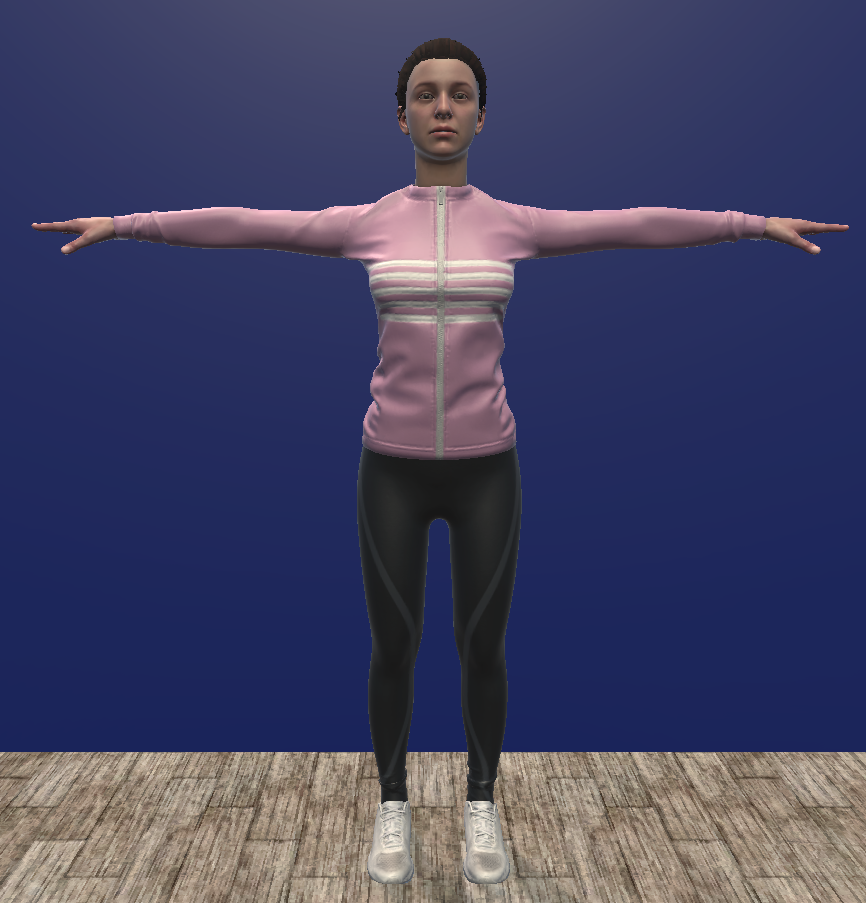
\includegraphics[width=\textwidth]{figures/Jade/Jade_Default.png}
    \caption{Jade (Mixamo) — photorealistic baseline used for initial NPR technique development.}
    \label{fig:jade_default}
  \end{subfigure}
  \hfill
  \begin{subfigure}[b]{0.45\textwidth}
    \centering
    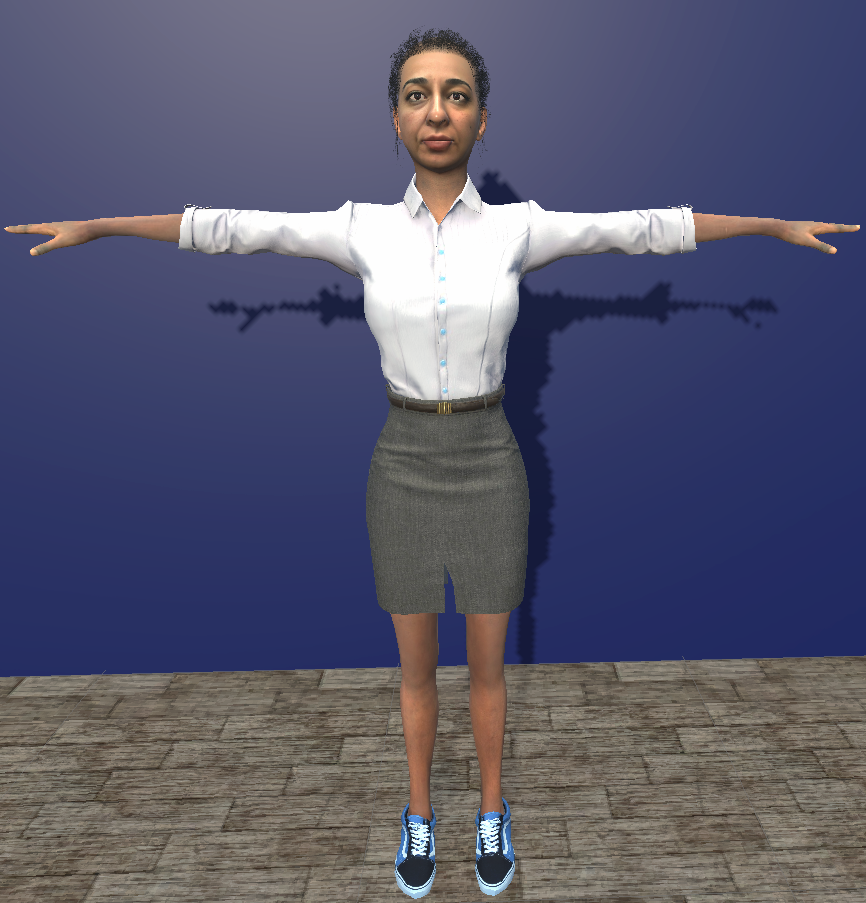
\includegraphics[width=\textwidth]{figures/Avaturn/avaturn_Default.png}
    \caption{Avaturn avatar — AI-reconstructed from a photograph, used as the primary platform for the user study.}
    \label{fig:avaturn_default}
  \end{subfigure}
  \caption{Default appearances of the two primary avatar platforms used in this thesis.}
  \label{fig:avatar_platforms}
\end{figure}

\section{NPR Technique Design}
\label{sec:technique_design}

The NPR stylisation techniques were developed through an iterative process in which each technique responds to a specific observed limitation of its predecessor. Development began on the Mixamo platform, where shader access is unrestricted, then continued within the Meta SDK environment where hook constraints shaped several implementation decisions, and was finally validated on Avaturn. What follows is a conceptual overview of each technique's motivation and visual behaviour across the three platforms. Full implementation details are provided in~\Cref{ch:implementation}.

\subsection{Shared Rendering Structure}
\label{sec:shared_structure}

All techniques share a common two-pass rendering structure. The first pass is a dedicated silhouette outline pass; the second is the main forward-lit pass in which the technique-specific NPR surface effect is computed.

The silhouette outline is generated using the inverted hull method~\cite{lake2000, isenberg2003}. Front-face culling is enabled so that only back-facing geometry is rasterised. Every vertex is displaced outward along its world-space surface normal by a configurable distance, producing an enlarged shell around the avatar. When the main pass subsequently draws the front-facing surface over the interior, the shell remains visible only at the silhouette, appearing as a solid border of controllable thickness. The displacement is performed entirely in the vertex shader, requiring no mesh preprocessing. A depth bias prevents z-fighting where the expanded shell intersects the original geometry at similar depth values.

A consistent challenge across all passes is handling semitransparent avatar geometry. Hair is typically represented as a set of flat cards with an alpha-masked texture: each card is a rectangular polygon, and the hair shape is defined by discarding fragments whose alpha value falls below a threshold. Eyelashes and eyebrow geometry use the same cutout approach. Without correct alpha handling in the outline pass, the expanded hull would be drawn across the full rectangular extent of each hair card, producing a solid rectangular border instead of a border that follows the hair silhouette. Both the outline pass and the main forward-lit pass therefore sample the base colour texture alpha channel and discard fragments below the cutout threshold before any shading or displacement is applied. This ensures that outline thickness and surface effects are consistent between the opaque body geometry and the alpha-masked regions, and that transparent areas such as the interior of the eye cornea are handled correctly.

\subsection{V1 — Toon Shading}
\label{sec:v1}

The first technique establishes the toon shading baseline. The shared silhouette outline pass provides the outer border; the forward-lit pass replaces the standard Lambertian shading with a quantized diffuse model that produces the flat, banded appearance of cartoon rendering.

The toon shading model replaces the continuous Lambertian diffuse term with a stepped function~\cite{gooch1998}. The dot product of the light direction and surface normal is divided into a configurable number of discrete bands. Each individual band boundary receives an independent smoothstep transition of controllable width, so that normal jitter near a boundary causes a narrow localised blend rather than snapping the entire surface patch between steps — a more temporally stable approach than applying a single global threshold. A Fresnel rim lighting term, approximated using Schlick's formulation~\cite{schlick1994}, brightens surface regions facing perpendicular to the viewer. A constant ambient term prevents fully shadowed regions from collapsing to black.

The Meta SDK platform implementation follows a different architectural path from the Mixamo and Avaturn variants. Rather than operating on a raw diffuse dot product, it receives the fully composited PBR output of the SDK renderer — including subsurface scattering, anisotropic hair shading, eye glints, and image-based lighting — and posterises the RGB result directly. The cel-shaded colour therefore retains the physical material quality of the underlying renderer; the stylisation abstracts its tonal range without discarding the lighting information already encoded in it.

The limitation of V1 is that the outer silhouette remains the only visible boundary. Internal surface features — facial features, clothing seams, surface creases — produce no edge signal.

\begin{figure}[H]
  \centering
  \missingfigure[figwidth=\textwidth]{V1 (Toon Shading + Geometry Outline): Mixamo (left) / Meta SDK (centre) / Avaturn (right)}
  \caption{V1 (Toon Shading with Geometry-Based Outlines) across the three avatar platforms.}
  \label{fig:v1_platforms}
\end{figure}

\subsection{V2 — X-Toon Extended Toon Shading}
\label{sec:v2}

The second technique extends the toon shading model of V1 using the X-Toon approach proposed by Barla et al.~\cite{barla2006}. Standard toon shading indexes a one-dimensional ramp texture using the Lambertian dot product between the surface normal and the light direction, which determines the diffuse shading band. X-Toon replaces this with a two-dimensional ramp texture, introducing a second lookup axis that encodes an additional scene property. In this implementation the second axis encodes the fragment's distance from the camera, allowing the shading response to vary with depth. Regions close to the viewer receive a standard toon diffuse treatment; at greater distances the ramp shifts the shading response, producing a depth-dependent variation in tone that increases perceived depth and separation between overlapping body parts.

The key advantage over V1 is expressive control over how depth reads in the final image: the designer can tune the 2D ramp texture to lighten or darken distant regions, emphasise contour separation at a chosen distance, or introduce atmospheric depth without any additional geometry. The limitation is that neither the toon model nor the 2D ramp produces any signal for interior surface detail such as facial features or clothing seams. The only visible boundary remains the outer silhouette from the shared hull pass.

\begin{figure}[H]
  \centering
  \missingfigure[figwidth=\textwidth]{V2 (X-Toon Extended Toon Shading): Mixamo (left) / Meta SDK (centre) / Avaturn (right)}
  \caption{V2 (X-Toon Extended Toon Shading) across the three avatar platforms.}
  \label{fig:v2_platforms}
\end{figure}

\subsection{V3 — Screen-Space Normal Edge Detection}
\label{sec:v3}

The third technique introduces the first interior edge signal by detecting discontinuities in the interpolated surface normal across adjacent screen pixels. The GPU hardware intrinsics \texttt{ddx} and \texttt{ddy} expose the finite difference of any fragment-stage value across a two-by-two pixel quad at negligible cost, requiring no additional texture samples. Applying this to the world-space surface normal gives a gradient magnitude as defined in~\Cref{sec:background_normal_deriv}, which responds to creases, mesh boundaries, and regions of high curvature — features that are invisible to the toon shading approaches of V1 and V2. The computation adds no texture samples to the fragment shader and executes at near-zero additional cost relative to the surrounding lighting evaluation. The key limitation is that edge thickness is measured in screen pixels and therefore scales with camera distance, producing edges that grow thinner as the avatar recedes from the viewer.

\begin{figure}[H]
  \centering
  \missingfigure[figwidth=\textwidth]{V3 (Normal Edge Detection): Mixamo (left) / Meta SDK (centre) / Avaturn (right)}
  \caption{V3 (Screen-Space Normal Edge Detection) across the three avatar platforms.}
  \label{fig:v3_platforms}
\end{figure}

\subsection{V4 — Sobel Edge Detection}
\label{sec:v4}

The fourth technique applies the Sobel operator to the avatar's diffuse albedo texture to extract colour boundaries. This captures clothing patterns, facial contour transitions, and other surface details that have no geometric counterpart. Two artefact types arise. First, UV seam boundaries produce spurious high-gradient spikes where the texture wraps discontinuously across a seam. Second, uniform skin regions produce over-detection at low thresholds because the subtle colour variation in skin tones registers as a weak but persistent edge signal. The first artefact is suppressed by a luminance range check that rejects detections where the spread of neighbourhood luminance values exceeds a configurable limit. The second is addressed by a skin classification computed per pixel based on HSV saturation that applies a stricter detection threshold in regions of low saturation.

\begin{figure}[H]
  \centering
  \missingfigure[figwidth=\textwidth]{V4 (Sobel Edge Detection): Mixamo (left) / Meta SDK (centre) / Avaturn (right)}
  \caption{V4 (Sobel Edge Detection with adaptive skin thresholding) across the three avatar platforms.}
  \label{fig:v4_platforms}
\end{figure}

\subsection{V5 — Gaussian Prefiltered Sobel}
\label{sec:v5}

The fifth technique addresses edge noise by approximating Gaussian pre-filtering before gradient computation. Following the observation of Marr and Hildreth~\cite{marr1980} that stable edge detection requires prior low-pass smoothing, this version samples the diffuse texture at a grid of offset positions and computes a weighted average before applying the Sobel operator. The smoothing reduces noise and suppresses fine texture artefacts, producing cleaner edge lines. The trade-off is a substantially higher per-fragment sample count. A further limitation is that the smoothing is spatially uniform: it softens genuine structural boundaries alongside artefacts, producing edges that are smoother in aggregate but not more selective in what they mark.

\begin{figure}[H]
  \centering
  \missingfigure[figwidth=\textwidth]{V5 (Gaussian Sobel): Mixamo (left) / Meta SDK (centre) / Avaturn (right)}
  \caption{V5 (Gaussian Prefiltered Sobel) across the three avatar platforms.}
  \label{fig:v5_platforms}
\end{figure}

\subsection{V6 — Hierarchical Edge Detection with Multiple Cues}
\label{sec:v6}

The sixth technique fuses three independent edge cues through weighted combination, addressing the limitation that no single cue reliably captures all visually meaningful boundaries. A depth proximity layer uses derivatives in screen space of the camera-to-fragment distance to detect silhouette-level boundaries. A normal layer detects surface crease edges from normal discontinuities. A colour layer applies the Roberts Cross operator to the diffuse texture to capture painted detail boundaries. The three layers are blended using weights per layer that can be adjusted at runtime, allowing the visual balance between silhouette, crease, and texture edges to be controlled interactively. This technique detects the broadest range of edge types of any approach developed to this point.

\begin{figure}[H]
  \centering
  \missingfigure[figwidth=\textwidth]{V6 (Hierarchical Multi-Cue): Mixamo (left) / Meta SDK (centre) / Avaturn (right)}
  \caption{V6 (Hierarchical Edge Detection with Multiple Cues) across the three avatar platforms.}
  \label{fig:v6_platforms}
\end{figure}

\subsection{V7 — Kuwahara Painterly Filter}
\label{sec:v7}

Rather than drawing explicit edge lines, the seventh technique applies the isotropic Kuwahara filter to the rendered surface colour to produce a painterly abstraction. For each fragment, four overlapping quadrant regions are sampled; the output is set to the mean colour of whichever quadrant has the lowest local variance. Uniform surface regions are smoothed toward a flat painterly fill, while region boundaries are sharpened implicitly because the selected quadrant is always the one that falls cleanly on one side of the boundary. This is the only technique in this thesis that does not produce explicit ink lines; the abstraction operates entirely through regional colour smoothing.

\begin{figure}[H]
  \centering
  \missingfigure[figwidth=\textwidth]{V7 (Kuwahara): Mixamo (left) / Meta SDK (centre) / Avaturn (right)}
  \caption{V7 (Kuwahara Painterly Filter) across the three avatar platforms.}
  \label{fig:v7_platforms}
\end{figure}

\subsection{V8 — Kuwahara with Sobel Edges}
\label{sec:v8}

The eighth technique combines the painterly region abstraction of V7 with the ink-line edges of V4. The Kuwahara pass is applied first to produce smooth filled regions, and Sobel edges are composited on top to add explicit contour lines. The result is a comic-book aesthetic: flat coloured regions separated by drawn boundaries. Because the edge detection runs on the abstracted Kuwahara output rather than the original diffuse texture, the lines reflect the abstracted region structure rather than every fine texture variation.

\begin{figure}[H]
  \centering
  \missingfigure[figwidth=\textwidth]{V8 (Kuwahara + Sobel): Mixamo (left) / Meta SDK (centre) / Avaturn (right)}
  \caption{V8 (Kuwahara with Sobel Edges) across the three avatar platforms.}
  \label{fig:v8_platforms}
\end{figure}

\subsection{V9 — Composite: Kuwahara, Gaussian Sobel, and Hierarchical}
\label{sec:v9}

The ninth technique chains all three main abstraction strategies into a single pipeline. The Kuwahara filter is applied first to produce the painterly base. Gaussian prefiltered Sobel edges are then composited to add smoothed colour boundary lines. Finally, the hierarchical multi-cue layer contributes depth, normal, and colour edges with independent weighting. This produces the richest visual output of any technique in the set, combining surface abstraction with two complementary edge detection strategies at the cost of the highest sample count per fragment of all techniques developed so far.

\begin{figure}[H]
  \centering
  \missingfigure[figwidth=\textwidth]{V9 (Composite): Mixamo (left) / Meta SDK (centre) / Avaturn (right)}
  \caption{V9 (Composite: Kuwahara, Gaussian Sobel, Hierarchical) across the three avatar platforms.}
  \label{fig:v9_platforms}
\end{figure}

\section{Technique Selection for the User Study}
\label{sec:technique_selection}

Following the iterative development phase, a single technique is selected for the NPR condition in the user study based on visual assessment across all three avatar platforms. Three criteria guide the selection. First, facial expression detail must remain readable under the stylisation, since the study measures trust responses to a speaking avatar. Second, the effect must be visually coherent across viewing distances, since the video scenarios are filmed at a fixed conversational distance. Third, the abstraction must be clearly distinct from the photorealistic baseline to ensure that any difference in trust ratings reflects a genuine perceptual response to the stylisation. The outcome of this assessment is documented in~\Cref{ch:evaluation}.

\section{User Study Design}
\label{sec:user_study}

\subsection{Objective and Hypotheses}
\label{sec:study_objective}

The user study addresses RQ3 by measuring how the visual representation of a speaker affects the perceived trustworthiness of their advice in a concrete decision situation. Three presentation conditions are compared: a real human speaker, a photorealistic Avaturn avatar, and an Avaturn avatar rendered with NPR stylisation. Two hypotheses are tested.

\textbf{H1:} Participants will rate the real-person condition as most trustworthy, establishing a human baseline against which avatar conditions can be compared.

\textbf{H2:} The NPR-stylised avatar will not be rated significantly less trustworthy than the photorealistic avatar, and may be rated more trustworthy if the photorealistic condition triggers uncanny valley discomfort.

\subsection{Conditions}
\label{sec:study_conditions}

The study compares three presentation conditions:

\begin{description}
  \item[C0 — Real Person:] A video recording of a real human speaker delivering the recommendation. This serves as the trust ceiling baseline.
  \item[C1 — Photorealistic Avatar:] The same speaker scenario rendered using a photorealistic Avaturn avatar with standard PBR shading. Facial expressions are driven by blendshape animation to match the delivery timing.
  \item[C2 — NPR Avatar:] The Avaturn avatar rendered with the NPR technique selected from the visual assessment as providing the best balance of abstraction and expressiveness.
\end{description}

\subsection{Scenarios}
\label{sec:study_scenarios}

Three video scenarios are designed to present naturalistic decisions in which the speaker's trustworthiness is relevant. Each scenario introduces a situation with two plausible options and shows the speaker recommending one. The scenarios are kept domain-neutral to avoid prior knowledge effects. After watching each video, participants rate how trustworthy they found the speaker's recommendation.

Scenario content, option framing, and speaker delivery are held constant across conditions; only the visual presentation of the speaker changes. The three scenarios are counterbalanced across conditions using a Latin square to control for scenario-condition order effects.

\subsection{Procedure and Measures}
\label{sec:study_procedure}

The study uses a within-subjects design. Each participant watches all three conditions across the three scenarios, with condition-scenario assignment randomised per participant. After each video, participants complete a short questionnaire including a trust rating scale and items from the Godspeed questionnaire~\cite{macdorman2006} assessing human-likeness and eeriness.

Within-subjects differences across the three conditions are analysed using a repeated-measures design. Pairwise comparisons between each avatar condition and the real-person baseline, and between the two avatar conditions, are conducted with Bonferroni correction. Effect sizes are reported as partial $\eta^2$.

\subsection{Ethical Considerations}
\label{sec:study_ethics}

The study was reviewed and approved by the University of Konstanz ethics committee. Participants provided written informed consent before participation. Data is anonymised at collection; no personally identifiable information is stored alongside questionnaire responses. Participation was voluntary with the right to withdraw at any time.
